\begin{comment}

Keywords:

    - The kind of data needed
    - Data example
    - Equipment
    - Filming process
    - Video to keypoints data conversion
    - Pose estimation
    - Software
    - Hardware
    - Process
    - Data produced and quality control
        

\end{comment}

As with most problems potentially solvable by implementing machine learning based solutions, the data to be explored and used to train machine learning models plays central part in our implementation. Although, machine learning promises to loosen the strictness of the data used in a system by trying to generalize and adapt the models themselves to the data, the quality of the initial data used to develop prototypes still directly influences the interpretation and value of the outcome. Interpretation of not only the outcome, but the entire solution is needed to have clear understanding of why certain outcomes exist, which in turn helps to spark discussion and spread knowledge gained during an experiment. The value of this work as a scientific paper, reusable by peers for new scientific experiments, is also directly influenced by the quality of the initial data. The author of this work is aware, that by choosing a very niche dataset he risks to reduce the social reach of this work and thereby stresses to point that he mainly wishes to contribute his finding to the human activity recognition domain and not necessarily to the specific sports domain of gymnastics.

The data acquisition chapter is split into two parts. First, the part explaining what kind and how much of data the author is collecting and the process behind it. The second part explains a more technical approach on how the initial data for the human activity recognition algorithm is acquired from recorded human motions and the tools used to do so.

\section{Recording Human Actions}

\subsection{Choosing Activities To Record}

When it comes to choosing difficult biomechanical activities performed by humans, gymnastics comes on the top of the list. Gymnastic feats don't require any additional equipment by humans, but physical strength, flexibility and kinesthetic awareness are a must to perform any of the skills demonstrated by elite athletes. Gymnastics is also special in its indisputable need for utilizing every part of the human body. All major muscle groups of an athlete need to be in superior condition to perform certain rotations, jumps and holds. So, many athletes start their career at a very young age.

Automatic recognition of human activity requires reference or training data to train our machine to recognize some gymnastic movements. The two activities chosen to prove the hypothesis of this paper are backflips and back handsprings. Figures \ref{example-of-backflip} and \ref{example-of-back-handspring} will hopefully give the reader a visual idea of backflips and back handsprings respectively.

\begin{figure*}
   \centering
\begin{tabular}{ccc}
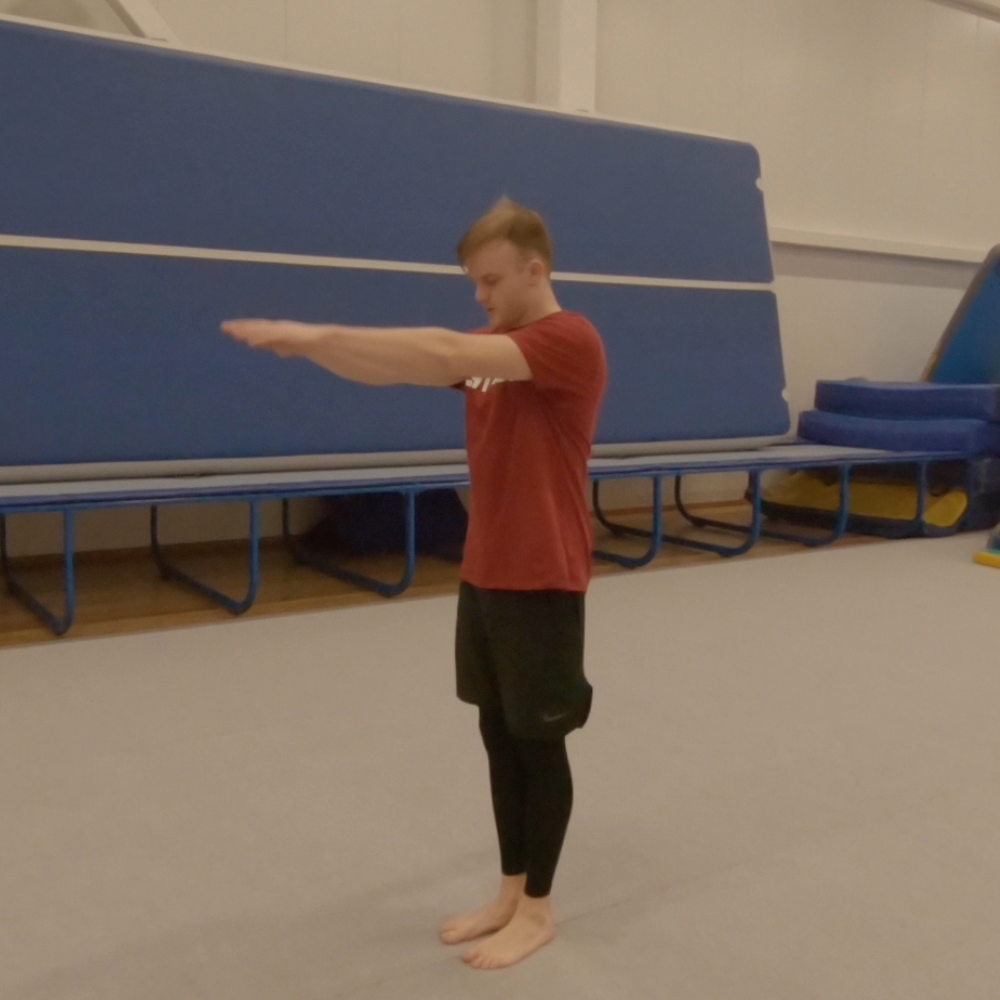
\includegraphics[width=5cm]{images/data-acquisition/example-backflip-part-1}&
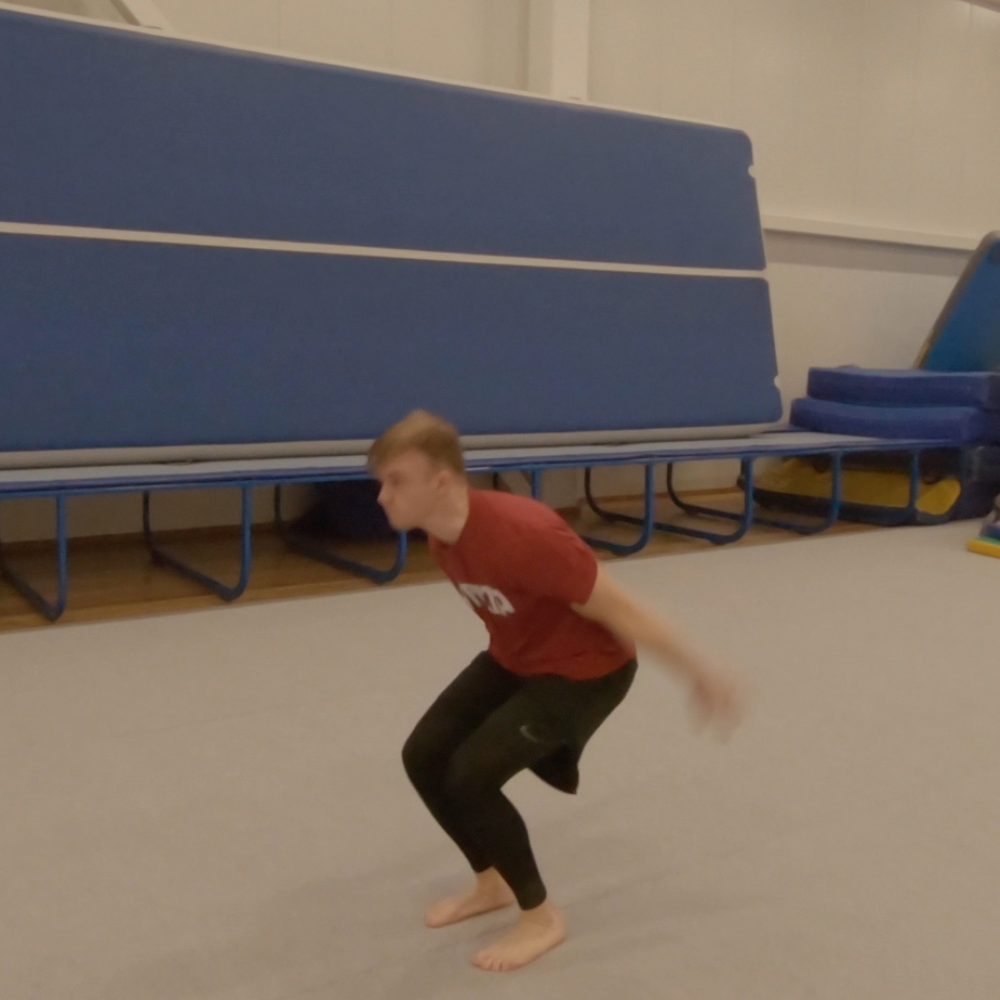
\includegraphics[width=5cm]{images/data-acquisition/example-backflip-part-2}&
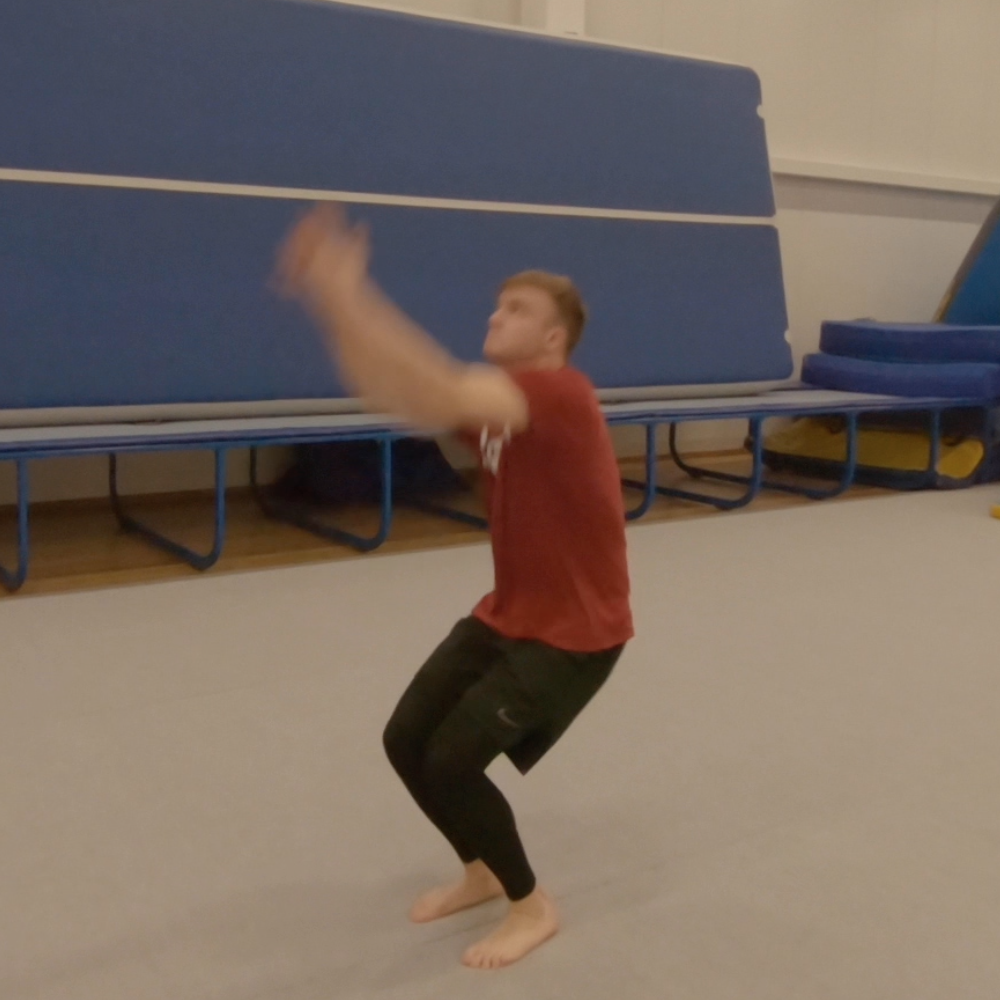
\includegraphics[width=5cm]{images/data-acquisition/example-backflip-part-3}\\
&
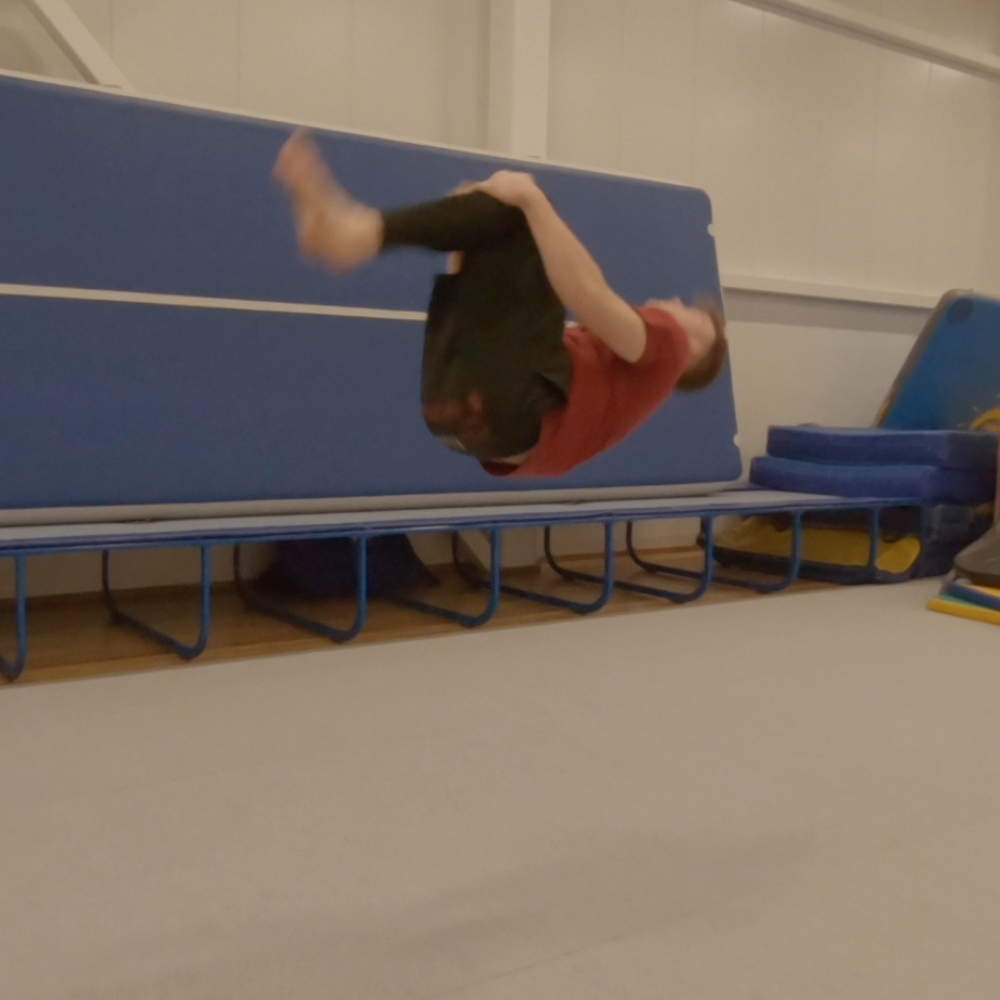
\includegraphics[width=5cm]{images/data-acquisition/example-backflip-part-4}&
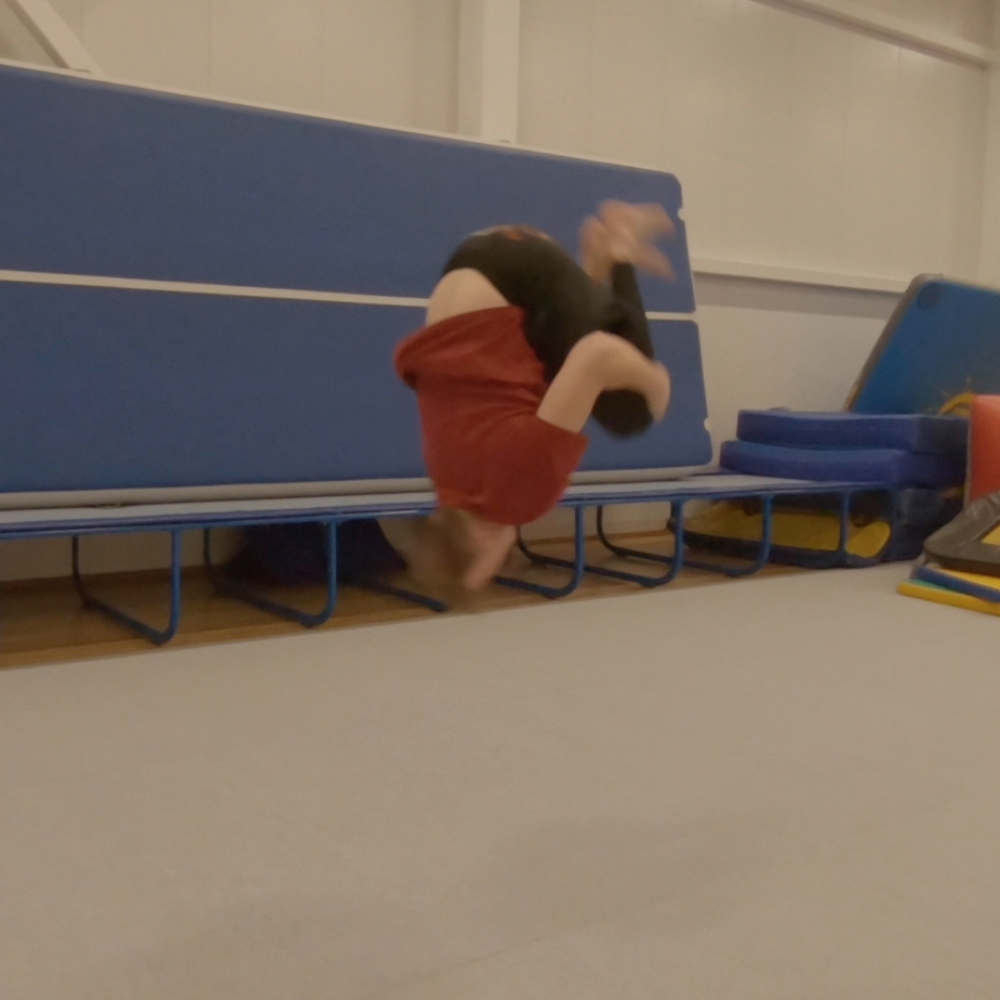
\includegraphics[width=5cm]{images/data-acquisition/example-backflip-part-5}\\
\end{tabular}
    \caption{Example of a backflip}
    \label{example-of-backflip}
\end{figure*}

\begin{figure*}
   \centering
\begin{tabular}{ccc}
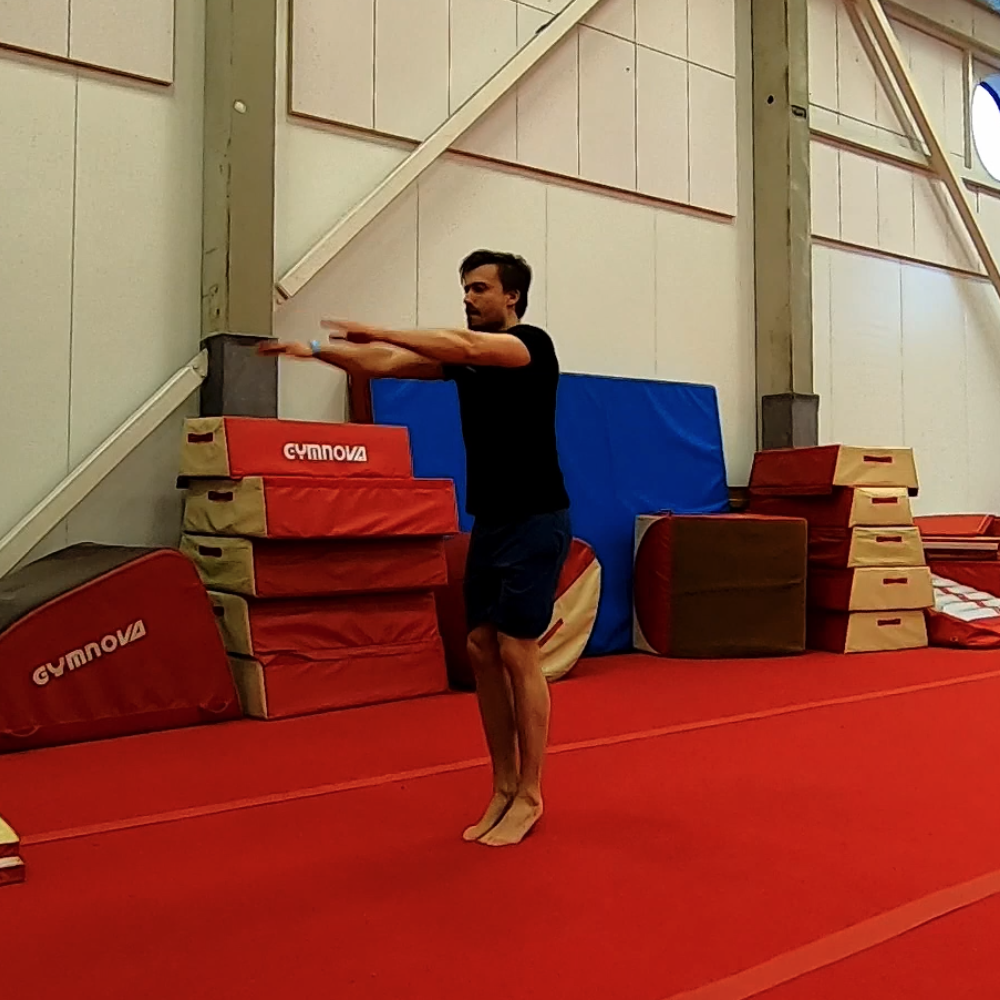
\includegraphics[width=5cm]{images/data-acquisition/example-flack-part-1}&
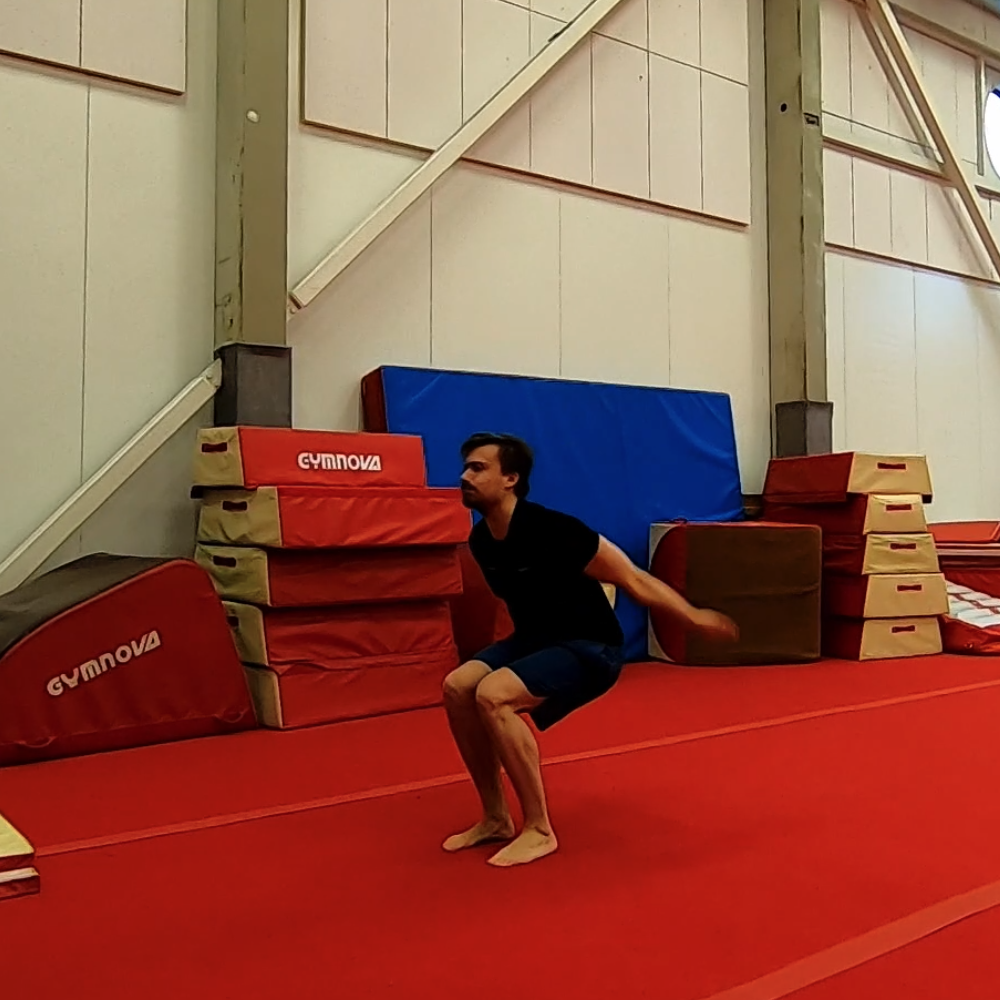
\includegraphics[width=5cm]{images/data-acquisition/example-flack-part-2}&
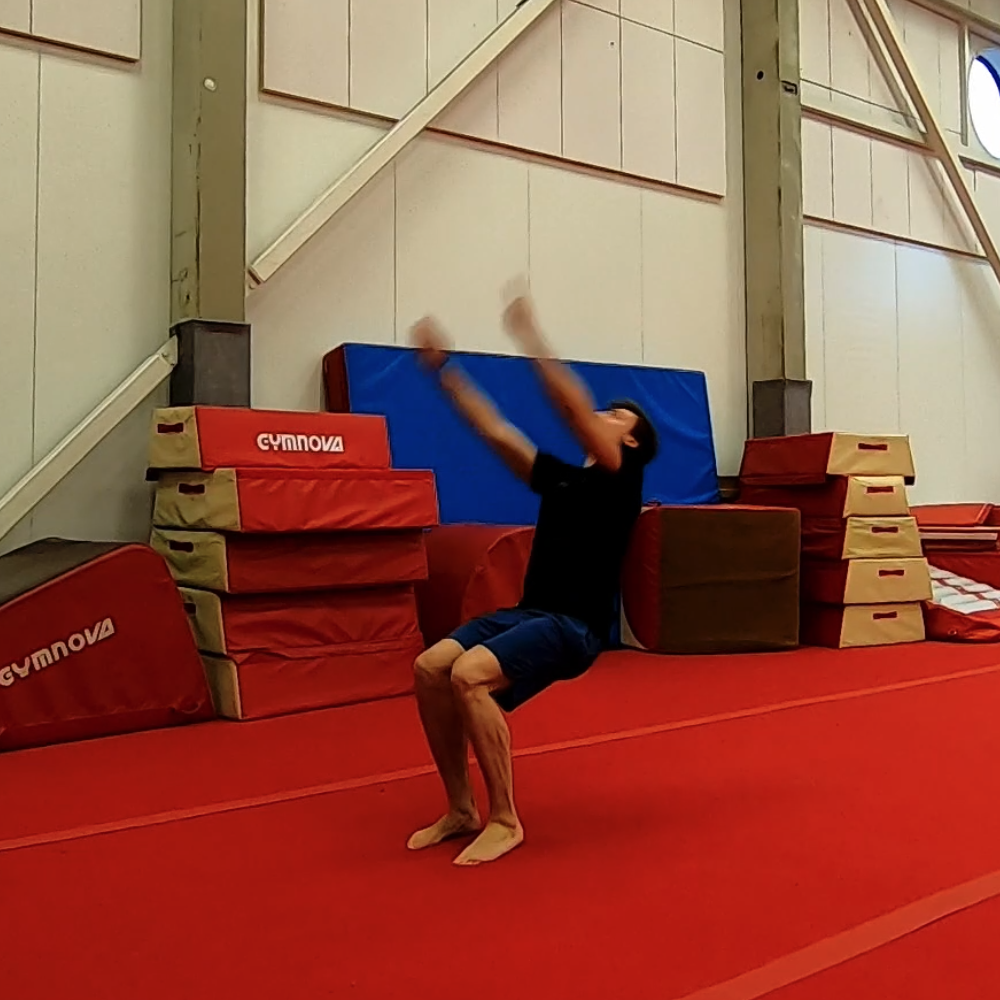
\includegraphics[width=5cm]{images/data-acquisition/example-flack-part-3}\\
&
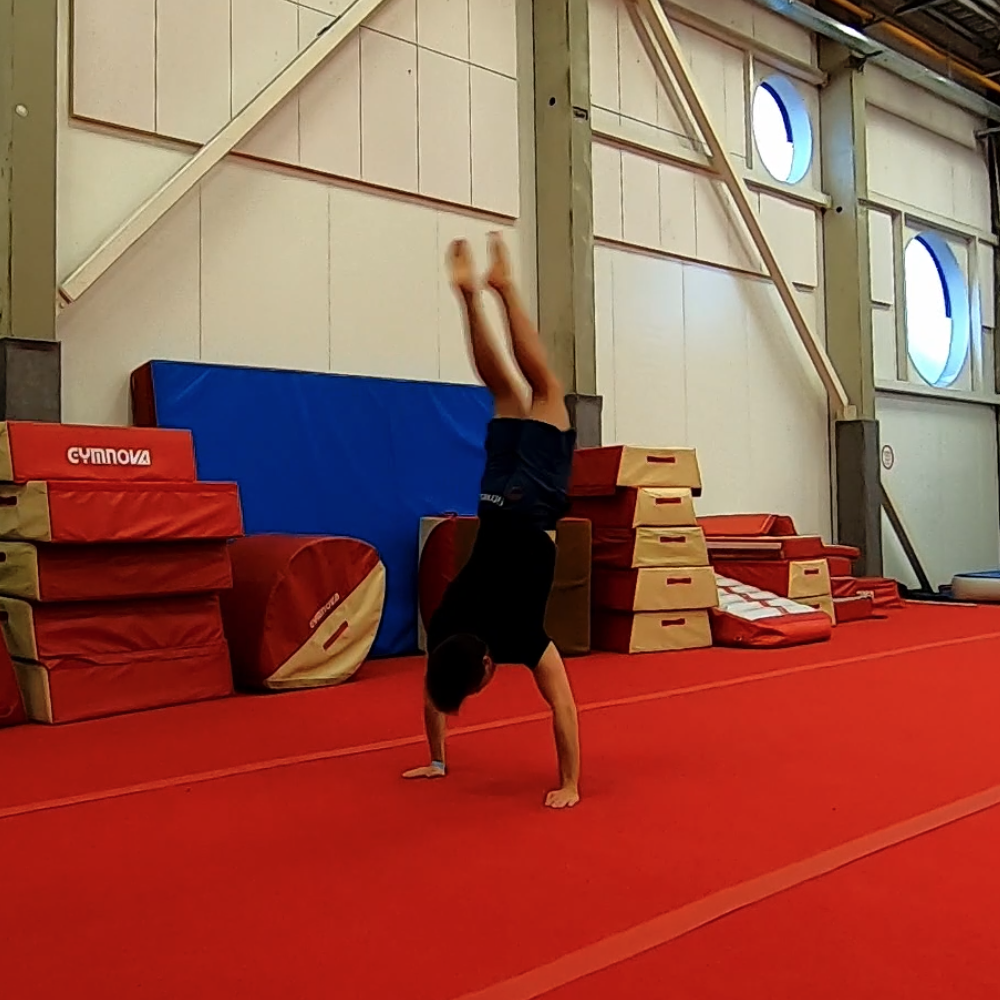
\includegraphics[width=5cm]{images/data-acquisition/example-flack-part-4}&
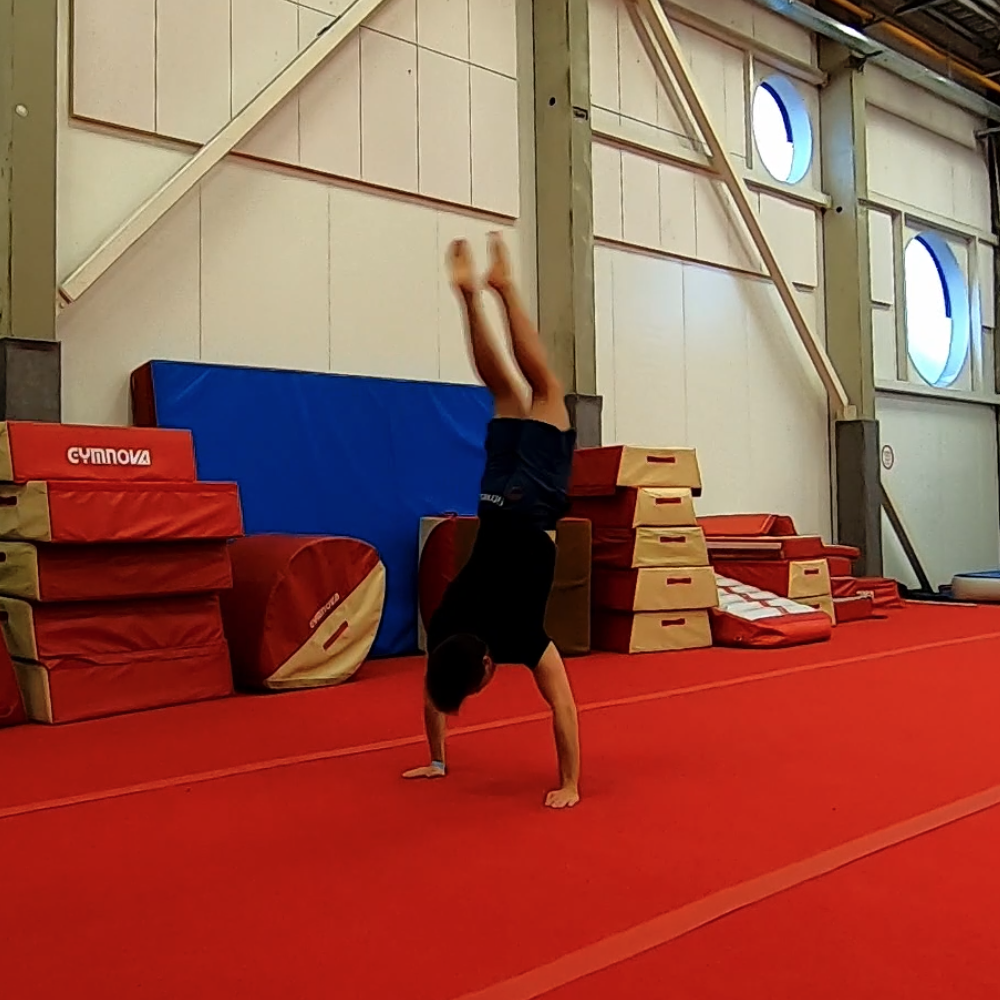
\includegraphics[width=5cm]{images/data-acquisition/example-flack-part-5}\\
\end{tabular}
    \caption{Examples of a back handspring}
    \label{example-of-back-handspring}
\end{figure*}

For each activity there needs to be specific start and end markers, so it could be easily recognized when the activity starts and when does it end.

The following is a detailed description of each activity and its parameters.

\subsection{Backflip}

A backflip is a sequence of body movements in which a person leaps into the air and rotates backwards over the body's horizontal axis. For the backflip, we mark the start of a backflip as the frame when athlete's both arms pass the horizontal line at shoulder level moving downwards and generating momentum. We mark the end of a backflip as the frame when both heels of the feet touch the ground again. We choose the heels of feet so we can include the amortization part of the landing phase of the backflip in the recording. The red bar in figure \ref{example-backflip-markers} demonstrates visual markers for trimming the sample recording to include only the activity under investigation. These markers were chosen by the author to the best of his knowledge of the domain as the clearest points for a human observer to recognize a backflip. Choosing different markers is a potential discussion topic for future improvements.

\begin{figure*}
   \centering
\begin{tabular}{cc}
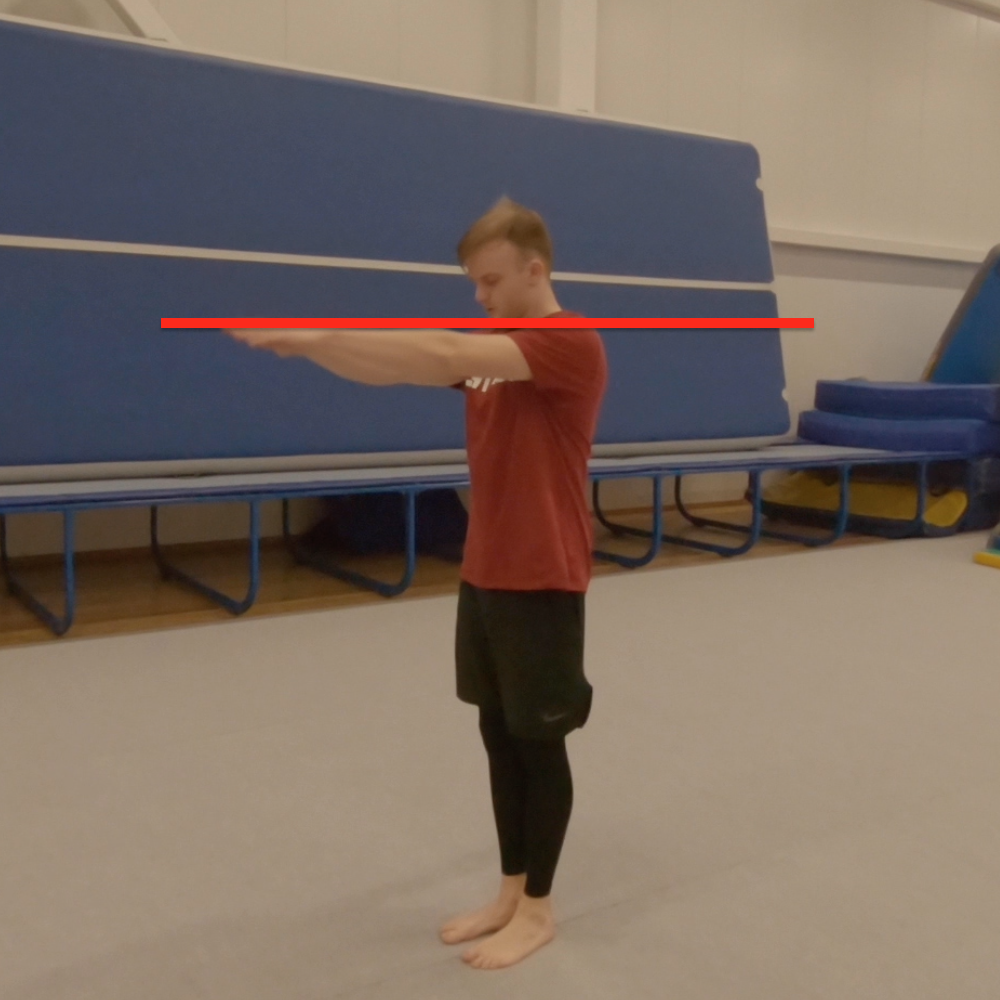
\includegraphics[width=5cm]{images/data-acquisition/example-backflip-marker-start}&
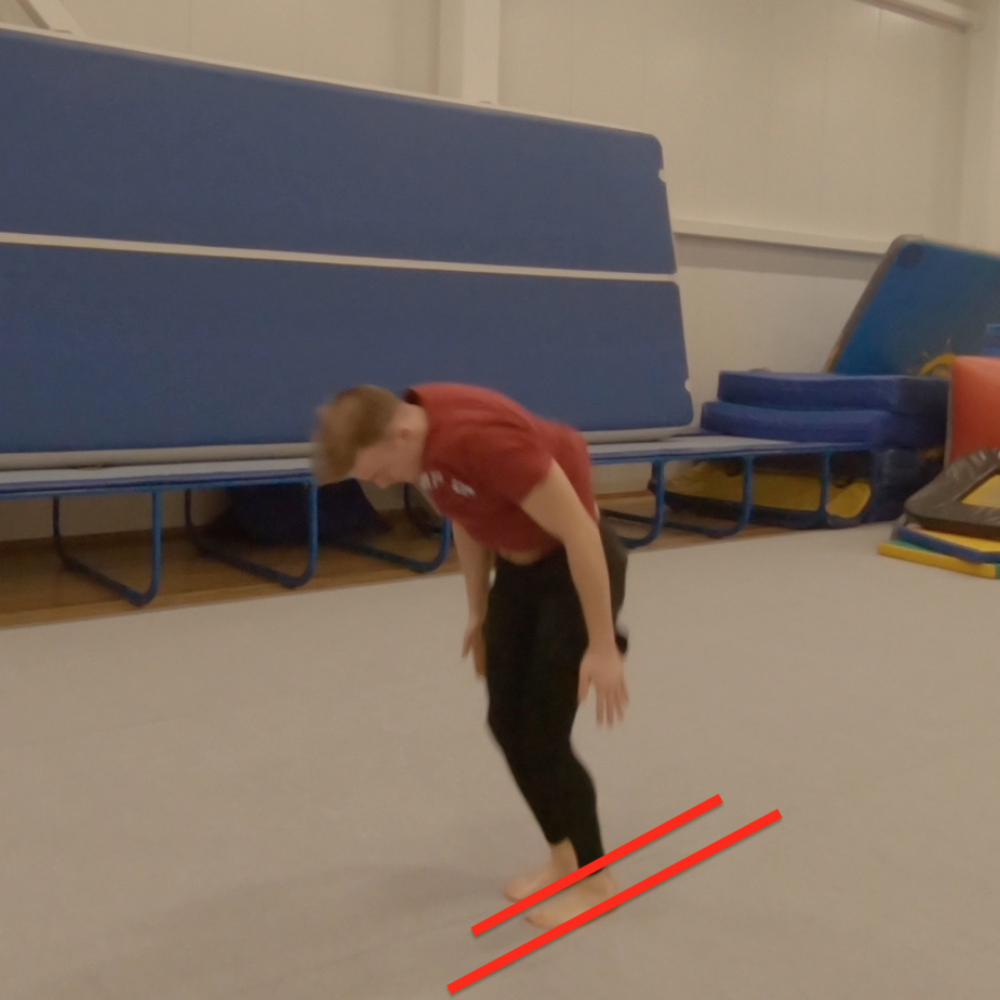
\includegraphics[width=5cm]{images/data-acquisition/example-backflip-marker-end}\\
\end{tabular}
    \caption{Start and end markers for covering the full duration of a backflip}
    \label{example-backflip-markers}
\end{figure*}

\subsection{Back Handspring}

TODO

\subsection{Recording Process}

Since these types of movements are performed for a duration of time, just still images of activities are not sufficient. We need the activities recorded in some kind of motion picture format. The device used to capture activities is a GoPro Hero7 Black, with the following basic settings:

* RES - 1080
* FPS - 60
* FOV - Linear
* Low Light - Auto
* Stabilization - Auto
* Protune - Off

Each activity is recorded as one still view from eye level angle fully showing the subjects body from head to toe.

\section{Estimating and Collecting Action Poses}















